% =====================================================================
%  Software Requirements Specification (SRS) v1
%  Lab 2: Problem Definition + SRS
%  Project: BusGo Microservices Bus Ticket Booking Platform
%  Compile on Overleaf with: pdfLaTeX
% =====================================================================
\documentclass[11pt,a4paper]{article}

% ---------- Packages ----------
\usepackage[utf8]{inputenc}
\usepackage[T1]{fontenc}
\usepackage{textcomp}
\usepackage{amsmath}
\usepackage{amssymb}
\usepackage[a4paper,margin=2.2cm]{geometry}
\usepackage{longtable}
\usepackage{array}
\usepackage{tabularx}
\usepackage{booktabs}
\usepackage{enumitem}
\usepackage[table]{xcolor}
\usepackage{ltablex}   % makes tabularx X-columns work inside longtable
\keepXColumns          % keep X columns expanding (don't convert to l)
\usepackage{titlesec}
\usepackage{fancyhdr}
\usepackage{graphicx}
\usepackage{tikz}
\usetikzlibrary{shapes.geometric, arrows.meta, positioning, fit, backgrounds}
\usepackage{hyperref}
\hypersetup{
    colorlinks=true,
    linkcolor=blue!55!black,
    urlcolor=blue!55!black,
    citecolor=blue!55!black,
    pdftitle={BusGo SRS v1},
    pdfauthor={Team T07}
}

% ---------- Colors ----------
\definecolor{busgoblue}{RGB}{20,80,150}
\definecolor{lightgray}{RGB}{240,240,240}
\definecolor{headergray}{RGB}{225,232,240}

% ---------- Section styling ----------
\titleformat{\section}{\color{busgoblue}\Large\bfseries}{\thesection}{0.6em}{}
\titleformat{\subsection}{\color{busgoblue!85!black}\large\bfseries}{\thesubsection}{0.5em}{}
\titleformat{\subsubsection}{\bfseries}{\thesubsubsection}{0.5em}{}

% ---------- Header / Footer ----------
\pagestyle{fancy}
\fancyhf{}
\lhead{\textcolor{busgoblue}{\small BusGo SRS v1.0}}
\rhead{\small Team T07}
\cfoot{\small Page \thepage\ of \pageref{LastPage}}
\renewcommand{\headrulewidth}{0.4pt}
\usepackage{lastpage}

% ---------- Table helpers ----------
\newcolumntype{Y}{>{\raggedright\arraybackslash}X}
\renewcommand{\arraystretch}{1.3}

% Reusable styled long-table header
\newcommand{\rowstyle}{\rowcolor{headergray}}

\begin{document}

% =====================================================================
%  TITLE PAGE
% =====================================================================
\begin{titlepage}
\centering
\vspace*{1.5cm}
{\color{busgoblue}\Huge\bfseries Software Requirements\\[0.3cm] Specification (SRS) v1\par}
\vspace{0.8cm}
{\Large\itshape Lab 2: Problem Definition + SRS\par}
\vspace{1.2cm}
\rule{\textwidth}{1.2pt}\\[0.4cm]
{\LARGE\bfseries BusGo — Microservices Bus Ticket Booking Platform\par}
\rule{\textwidth}{1.2pt}\\[1.2cm]

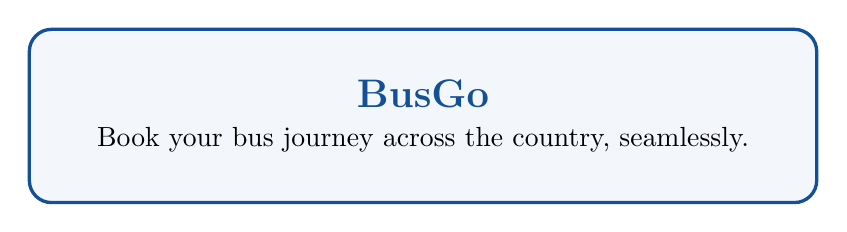
\begin{tikzpicture}
  \node[draw=busgoblue, line width=1.2pt, rounded corners=8pt, fill=busgoblue!5,
        minimum width=10cm, minimum height=2.2cm, align=center]{
    \Large\bfseries\color{busgoblue} BusGo\\[2pt]
    \normalsize Book your bus journey across the country, seamlessly.};
\end{tikzpicture}

\vspace{1.5cm}
{\large
\begin{tabular}{rl}
\textbf{Team:} & T07 \\
\textbf{Version:} & 1.0 \\
\textbf{Status:} & Draft \\
\textbf{Date:} & 28 June 2026 \\
\end{tabular}}

\vfill
{\small Prepared in accordance with the Lab 2 SRS Template.\par}
\end{titlepage}

\tableofcontents
\newpage

% =====================================================================
%  1. DOCUMENT CONTROL
% =====================================================================
\section{Document Control}

\subsection{Metadata}
\begin{tabularx}{\textwidth}{>{\bfseries}p{3.5cm} Y}
\toprule
Team & T07 \\
Project Name & BusGo — Microservices Bus Ticket Booking Platform \\
Repository URL & \url{https://github.com/TAUSEEF-01/Jaabo} \\
Version & 1.0 \\
Status & Draft \\
Date & 28 June 2026 \\
\bottomrule
\end{tabularx}

\subsection{Authors and Reviewers}
\begin{longtable}{>{\bfseries}p{3.2cm} p{3.2cm} p{4.6cm} p{2.6cm}}
\toprule
\rowstyle \textbf{Role} & \textbf{Name} & \textbf{ID / Email} & \textbf{Date} \\
\midrule
\endhead
Author & Md. Tauseef-Ur-Rahman & Roll 24 / satoru.gojo.thebest.01@gmail.com & 28-06-2026 \\
Author & Farzana Tasnim & Roll 14 & 28-06-2026 \\
Team Reviewer & Amina Islam & Roll 36 & 28-06-2026 \\
Team Reviewer & Tamzid Bin Tariq & Roll 48 & 28-06-2026 \\
\bottomrule
\end{longtable}

\subsection{Revision History}
\begin{longtable}{p{1.6cm} p{2.6cm} p{3.2cm} Y}
\toprule
\rowstyle \textbf{Version} & \textbf{Date} & \textbf{Author} & \textbf{Changes} \\
\midrule
\endhead
0.1 & 20-06-2026 & MD. Tauseef & Initial draft: problem definition and scope. \\
0.2 & 24-06-2026 & Team T07 & Added functional requirements, user stories, and data model. \\
0.3 & 26-06-2026 & Team T07 & Added NFRs, risk register, and manual test plan. \\
1.0 & 28-06-2026 & Team T07 & Consolidated review feedback; baseline release. \\
\bottomrule
\end{longtable}

% =====================================================================
%  2. PROBLEM DEFINITION
% =====================================================================
\section{Problem Definition}

\subsection{Problem Statement}
\textbf{What problem are we solving?}
Booking intercity bus tickets in many regional markets is still fragmented and unreliable.
Travellers must visit physical counters or juggle several operator-specific websites, none of
which expose a unified, real-time view of seat availability, fares, boarding points, or refund
policies. Bus operators, in turn, lack a single digital channel to publish trips, manage
inventory, run promotions, and reconcile payments. The result is overbooking, double-booked
seats, opaque cancellation rules, and a poor customer experience.

\medskip
\textbf{BusGo} solves this by providing a single, cloud-native, microservices-based platform
that unifies trip search, live seat selection, secure payment, e-ticketing, cancellations and
refunds, operator self-service, promotions, and administrative oversight behind one consistent
web experience and one API gateway.

\medskip
\textbf{Why does it matter?}
\begin{itemize}[leftmargin=1.4em]
  \item \textbf{For travellers:} a transparent, 24/7 self-service channel with real-time seat
        locking that eliminates double-booking and surprise cancellation charges.
  \item \textbf{For operators:} a low-cost digital storefront to reach customers, fill seats,
        and manage routes without building their own software.
  \item \textbf{For the business:} a scalable, independently deployable architecture (12
        services behind a Kong gateway) that can grow per-feature without monolithic rewrites.
\end{itemize}

\subsection{Target Users}
\begin{longtable}{p{3.2cm} Y Y}
\toprule
\rowstyle \textbf{User Group} & \textbf{Description} & \textbf{Main Needs} \\
\midrule
\endhead
Passengers (Customers) & End travellers searching, booking, and cancelling bus tickets via the web app. & Fast search, live seat map, secure payment, instant e-ticket, easy cancellation and refund tracking. \\
Bus Operators & Companies that own buses, define routes, schedule trips, and run promotions. & Manage buses/routes/trips, view bookings, run deals, monitor analytics and revenue. \\
Platform Administrators & Internal staff who govern the platform, onboard operators, and resolve disputes. & Operator approval, global oversight, broadcast notifications, audit trails. \\
Support / Operations Staff & Internal users handling cancellation reviews and customer issues. & Inspect bookings/payments, approve refunds, read audit logs. \\
\bottomrule
\end{longtable}

\subsection{Goals and Non-Goals}
\textbf{Goals}
\begin{itemize}[leftmargin=1.4em]
  \item Allow a passenger to search trips between two cities for a date and book a seat end-to-end.
  \item Guarantee no double-booking through time-bound seat locking in the Inventory service.
  \item Issue a verifiable QR e-ticket immediately after successful payment.
  \item Support cancellations with policy-driven refund calculation.
  \item Provide an operator portal for managing buses, routes, trips, and promo codes.
  \item Provide an admin portal with platform-wide oversight and an immutable audit log.
  \item Deliver the system as independently deployable services behind a single API gateway.
\end{itemize}

\textbf{Non-Goals}
\begin{itemize}[leftmargin=1.4em]
  \item Real money settlement: payment is handled via a \emph{mock} gateway, not a live PSP.
  \item Native mobile applications (iOS/Android) are out of scope for v1.
  \item Dynamic/surge pricing and AI-based seat recommendations.
  \item GPS live bus tracking and in-trip telemetry.
  \item Multi-language / multi-currency localisation beyond a single default locale.
\end{itemize}

% =====================================================================
%  3. SCOPE AND CONTEXT
% =====================================================================
\section{Scope and Context}

\subsection{In Scope}
\begin{itemize}[leftmargin=1.4em]
  \item User registration and authentication (phone + password, OTP verification, JWT, OAuth hook).
  \item City and trip search with availability filtering (\texttt{/api/search}).
  \item Live seat mapping, locking, and booking lifecycle (Inventory + Booking services).
  \item Mock payment processing and refund initiation (Payment service).
  \item Ticket generation with QR codes and downloadable PDF (Ticket service).
  \item Cancellation requests with refund calculation (Cancellation service).
  \item Operator self-service portal: buses, routes, trips, bookings, deals, analytics.
  \item Promo code / discount validation (Deals service).
  \item Admin portal and broadcast notifications (Admin + Notification services).
  \item System-wide action logging (Audit service).
  \item Event-driven cross-service workflows over Kafka; caching/sessions over Redis.
\end{itemize}

\subsection{Out of Scope}
\begin{itemize}[leftmargin=1.4em]
  \item Integration with real payment service providers and bank settlement (handled by mock Bank service).
  \item Loyalty/rewards programs and wallet balances.
  \item Third-party aggregator/reseller APIs and white-label embedding.
  \item Offline counter sales and POS hardware integration.
  \item Advanced fraud detection and KYC verification workflows.
\end{itemize}

\subsection{Assumptions and Constraints}
\textbf{Technical constraints}
\begin{itemize}[leftmargin=1.4em]
  \item Backend services are FastAPI (Python 3.12+); frontend is React + Vite + TypeScript.
  \item PostgreSQL 15 with a logical database per service (\texttt{auth\_db}, \texttt{booking\_db}, \dots).
  \item Kong API Gateway fronts all services on port 8000; services run on host ports 8101--8112.
  \item Redis for cache/session; Kafka for asynchronous inter-service events.
  \item Persistence via SQLAlchemy ORM using \texttt{Base.metadata.create\_all()} (no destructive migrations).
  \item Local orchestration via Docker Compose; observability via Prometheus, Grafana, and Loki.
\end{itemize}
\textbf{Organizational constraints}
\begin{itemize}[leftmargin=1.4em]
  \item Four-member student team; work delivered across timed lab milestones.
  \item No production cloud budget; deployment targets local/dev infrastructure.
\end{itemize}
\textbf{Timeline constraints}
\begin{itemize}[leftmargin=1.4em]
  \item Lab 2 deliverable (this SRS) due 28 June 2026.
  \item Manual test plan feeds Lab 3 peer review.
\end{itemize}

% =====================================================================
%  4. STAKEHOLDERS AND ROLES
% =====================================================================
\section{Stakeholders and Roles}

\subsection{Stakeholders}
\begin{longtable}{p{3.6cm} Y p{2.2cm}}
\toprule
\rowstyle \textbf{Stakeholder} & \textbf{Interest} & \textbf{Priority} \\
\midrule
\endhead
Passenger & Reliable booking, fair refunds, transparent fares. & High \\
Bus Operator & Higher seat occupancy, easy trip management, timely payouts. & High \\
Platform Owner (Business) & Transaction volume, platform reliability, operator growth. & High \\
Platform Administrator & Governance, dispute resolution, compliance via audit logs. & High \\
Support/Operations Staff & Efficient cancellation handling and issue resolution. & Medium \\
Development Team (T07) & Maintainable, testable, independently deployable services. & Medium \\
Payment/Bank Provider (mock) & Correct transaction and refund records. & Medium \\
\bottomrule
\end{longtable}

\subsection{User Roles and Permissions}
\begin{longtable}{p{2.6cm} Y Y}
\toprule
\rowstyle \textbf{Role} & \textbf{Description} & \textbf{Permissions} \\
\midrule
\endhead
CUSTOMER & Registered traveller using the public web app. & Search trips; lock/select seats; create bookings; pay; view/download tickets; request cancellations; apply promo codes; manage own profile. \\
OPERATOR & Verified bus operator staff. & CRUD on own buses/routes/trips; view own bookings; create/manage deals; send notifications to own customers; view own analytics. \\
ADMIN & Platform administrator. & Onboard/deactivate operators; global read across services; broadcast notifications; view audit logs; override/cancel bookings; manage platform-wide deals. \\
SUPPORT & Operations staff (subset of admin). & View bookings/payments; review and approve/reject cancellation requests; read audit logs. \\
\bottomrule
\end{longtable}

% =====================================================================
%  5. FUNCTIONAL REQUIREMENTS
% =====================================================================
\section{Functional Requirements}

Requirement ID format: \texttt{FR-T07-\#\#\#}. Priority uses MoSCoW: \textbf{M}ust, \textbf{S}hould,
\textbf{C}ould, \textbf{W}on't (this release). Each requirement is atomic and testable.

\begin{longtable}{p{1.9cm} p{2.2cm} Y p{0.9cm} Y}
\toprule
\rowstyle \textbf{Req ID} & \textbf{Feature} & \textbf{Requirement Statement} & \textbf{Pri} & \textbf{Acceptance Criteria} \\
\midrule
\endhead
FR-T07-001 & Registration & The system shall allow a new user to register with full name, unique phone, email, and password. & M & Account created; duplicate phone rejected with 409; password stored as hash. \\
FR-T07-002 & OTP Verify & The system shall verify a phone number via a time-limited OTP. & M & Valid OTP within expiry verifies account; expired/used OTP rejected. \\
FR-T07-003 & Login (JWT) & The system shall authenticate users with phone + password and issue a JWT access and refresh token. & M & Valid credentials return tokens; invalid return 401; refresh token rotates. \\
FR-T07-004 & City Search & The system shall let users search for origin/destination cities. & M & Partial query returns matching cities; empty query handled gracefully. \\
FR-T07-005 & Trip Search & The system shall return available trips for a given origin, destination, and journey date. & M & Results list operator, departure, fare, and seats available; no past-date trips. \\
FR-T07-006 & Seat Map & The system shall display a live seat map for a selected trip showing AVAILABLE/LOCKED/BOOKED. & M & Seat statuses reflect inventory in real time. \\
FR-T07-007 & Seat Lock & The system shall lock selected seats for a bounded time window during booking. & M & Locked seats unavailable to others until expiry; lock auto-releases on timeout. \\
FR-T07-008 & Passenger Details & The system shall capture passenger details and boarding/dropping points per booking. & M & Booking rejects missing mandatory passenger fields. \\
FR-T07-009 & Create Booking & The system shall create a booking in INITIATED state with an idempotency key. & M & Duplicate idempotency key returns the original booking, not a new one. \\
FR-T07-010 & Apply Promo & The system shall validate and apply a promo code to compute discount. & S & Valid code reduces fare; invalid/expired code rejected with reason. \\
FR-T07-011 & Payment & The system shall process payment for a booking via the mock gateway. & M & Successful payment moves booking to CONFIRMED; failure leaves seats releasable. \\
FR-T07-012 & Ticket Issue & The system shall issue a QR e-ticket on successful payment. & M & Ticket has unique QR data and downloadable PDF; one ticket per booking. \\
FR-T07-013 & View Bookings & The system shall list a user's bookings with current status. & M & Bookings shown newest-first with status and fare. \\
FR-T07-014 & Cancellation & The system shall allow a user to request cancellation of a confirmed booking. & M & Request recorded as PENDING; refund amount computed per policy. \\
FR-T07-015 & Refund & The system shall initiate a refund for an approved cancellation. & S & Refund record created with estimated days; booking marked CANCELLED. \\
FR-T07-016 & Operator Bus Mgmt & The system shall let operators create, update, and deactivate buses. & M & Bus persisted with unique registration; deactivated bus excluded from new trips. \\
FR-T07-017 & Operator Route Mgmt & The system shall let operators define routes with boarding/dropping points. & M & Route saved with origin, destination, and distance. \\
FR-T07-018 & Operator Trip Mgmt & The system shall let operators schedule trips with fare and seat capacity. & M & Trip created as SCHEDULED; seat inventory generated for the trip. \\
FR-T07-019 & Operator Deals & The system shall let operators create promo codes for their trips. & S & Deal saved with validity window and discount; visible to eligible customers. \\
FR-T07-020 & Operator Analytics & The system shall show an operator revenue and bookings summary. & C & Dashboard renders totals for the operator's trips. \\
FR-T07-021 & Notifications & The system shall send booking/cancellation notifications to users. & S & Confirmation notification generated on CONFIRMED booking. \\
FR-T07-022 & Admin Operator Mgmt & The system shall let admins onboard and deactivate operators. & M & Operator activation toggled; deactivated operator trips hidden. \\
FR-T07-023 & Admin Broadcast & The system shall let admins broadcast notifications to user segments. & C & Broadcast recorded and delivered to targeted users. \\
FR-T07-024 & Audit Log & The system shall record key actions in an immutable audit log. & S & Each create/update/cancel writes an audit entry with actor and timestamp. \\
FR-T07-025 & Profile Mgmt & The system shall let users view and update their profile. & S & Updated fields persist; phone change re-triggers verification. \\
FR-T07-026 & API Gateway Routing & The system shall route all client traffic through the Kong gateway. & M & Requests reach correct service via \texttt{/api/<service>/*} routes. \\
FR-T07-027 & Health Checks & The system shall expose a health endpoint per service. & S & \texttt{/health} returns 200 when service and its dependencies are ready. \\
\bottomrule
\end{longtable}

% =====================================================================
%  6. USER STORIES AND USE CASES
% =====================================================================
\section{User Stories and Use Cases}

\subsection{User Stories}
\begin{longtable}{p{2.1cm} p{1.9cm} Y Y Y}
\toprule
\rowstyle \textbf{Story ID} & \textbf{As a...} & \textbf{I want...} & \textbf{So that...} & \textbf{Acceptance Criteria} \\
\midrule
\endhead
US-T07-001 & Passenger & to register with my phone number & I can access the platform & Account created and OTP sent. \\
US-T07-002 & Passenger & to verify my phone with an OTP & my account is trusted & Valid OTP marks account verified. \\
US-T07-003 & Passenger & to log in securely & I can access my bookings & Correct credentials return a JWT. \\
US-T07-004 & Passenger & to search trips between two cities on a date & I can plan my journey & Matching trips with fares are listed. \\
US-T07-005 & Passenger & to view a live seat map & I can pick my preferred seat & Seat statuses are accurate. \\
US-T07-006 & Passenger & seats I select to be held briefly & no one else takes them while I pay & Selected seats are locked until expiry. \\
US-T07-007 & Passenger & to enter passenger and boarding details & my ticket is correct & Booking stores passenger data. \\
US-T07-008 & Passenger & to apply a promo code & I pay a lower fare & Valid code reduces total fare. \\
US-T07-009 & Passenger & to pay for my booking & my seat is confirmed & Successful payment confirms booking. \\
US-T07-010 & Passenger & to receive a QR e-ticket & I can board the bus & Ticket with QR is issued and downloadable. \\
US-T07-011 & Passenger & to see all my bookings & I can track my trips & Bookings list shows status. \\
US-T07-012 & Passenger & to cancel a booking & I can get a refund when plans change & Cancellation request is recorded with refund amount. \\
US-T07-013 & Passenger & to track my refund status & I know when money returns & Refund shows status and estimated days. \\
US-T07-014 & Passenger & to manage my profile & my details stay current & Profile updates persist. \\
US-T07-015 & Operator & to add my buses & I can schedule trips on them & Bus saved with unique registration. \\
US-T07-016 & Operator & to define routes with stops & customers see boarding points & Route saved with stops. \\
US-T07-017 & Operator & to schedule trips with fares & customers can book them & Trip created and bookable. \\
US-T07-018 & Operator & to create promo codes & I can attract more bookings & Deal active within its validity window. \\
US-T07-019 & Operator & to view bookings on my trips & I can plan operations & Operator sees own trip bookings. \\
US-T07-020 & Operator & to see revenue analytics & I can track performance & Dashboard shows totals. \\
US-T07-021 & Admin & to approve operators & only legitimate operators sell tickets & Operator activation toggled. \\
US-T07-022 & Admin & to broadcast notifications & I can inform users of changes & Broadcast delivered to targets. \\
US-T07-023 & Admin & to view audit logs & I can investigate issues & Audit entries are searchable. \\
US-T07-024 & Support & to review cancellation requests & refunds are fair and correct & Request approved/rejected with reason. \\
\bottomrule
\end{longtable}

\subsection{Critical Use Cases}

\subsubsection*{UC-1: Book a Bus Ticket (End-to-End)}
\textbf{Actor:} Passenger (CUSTOMER).\\
\textbf{Preconditions:} User is registered, verified, and logged in; at least one matching trip exists.\\
\textbf{Main flow:}
\begin{enumerate}[leftmargin=1.6em]
  \item User searches origin, destination, and journey date.
  \item System returns available trips; user selects one.
  \item System displays the live seat map; user selects available seat(s).
  \item Inventory service locks the seats for the configured window.
  \item User enters passenger and boarding/dropping details.
  \item Booking service creates a booking (INITIATED) with an idempotency key.
  \item User optionally applies a valid promo code; fare is recomputed.
  \item User pays via the mock Payment service.
  \item On success, booking moves to CONFIRMED and the Ticket service issues a QR e-ticket.
  \item Notification service sends a booking confirmation.
\end{enumerate}
\textbf{Alternate / exception flow:}
\begin{itemize}[leftmargin=1.6em]
  \item 4a. Selected seat already locked/booked $\rightarrow$ system prompts re-selection.
  \item 7a. Invalid/expired promo $\rightarrow$ discount rejected with reason; user may retry.
  \item 8a. Payment fails or seat lock expires $\rightarrow$ booking not confirmed; seats released.
\end{itemize}
\textbf{Postconditions:} A CONFIRMED booking, a payment record, and a valid e-ticket exist; seats are BOOKED.

\subsubsection*{UC-2: Cancel a Booking and Process Refund}
\textbf{Actor:} Passenger; reviewed by Support/Admin.\\
\textbf{Preconditions:} User has a CONFIRMED booking eligible for cancellation.\\
\textbf{Main flow:}
\begin{enumerate}[leftmargin=1.6em]
  \item User opens a confirmed booking and requests cancellation with a reason.
  \item Cancellation service computes refund amount per policy and records a PENDING request.
  \item Support/Admin reviews and approves the request.
  \item Payment service initiates a refund with estimated processing days.
  \item Booking is marked CANCELLED; seats are released back to inventory.
  \item Notification service informs the user.
\end{enumerate}
\textbf{Alternate / exception flow:}
\begin{itemize}[leftmargin=1.6em]
  \item 3a. Request rejected $\rightarrow$ status REJECTED with rejection reason; no refund.
  \item 2a. Booking past cancellation cutoff $\rightarrow$ refund amount is zero per policy.
\end{itemize}
\textbf{Postconditions:} Booking CANCELLED; refund record created; seats AVAILABLE again.

\subsubsection*{UC-3: Operator Schedules a Trip}
\textbf{Actor:} Operator (OPERATOR).\\
\textbf{Preconditions:} Operator is active and has at least one active bus and route.\\
\textbf{Main flow:}
\begin{enumerate}[leftmargin=1.6em]
  \item Operator selects a bus and route and sets departure/arrival times, fare, and capacity.
  \item Operator service creates the trip in SCHEDULED state.
  \item Inventory service generates seat inventory for the trip.
  \item Trip becomes searchable to customers.
\end{enumerate}
\textbf{Alternate / exception flow:}
\begin{itemize}[leftmargin=1.6em]
  \item 1a. Inactive bus/route selected $\rightarrow$ trip creation rejected.
  \item 2a. Overlapping trip on the same bus $\rightarrow$ conflict warning.
\end{itemize}
\textbf{Postconditions:} A bookable SCHEDULED trip with generated seat inventory exists.

% =====================================================================
%  7. DATA REQUIREMENTS
% =====================================================================
\section{Data Requirements}

\subsection{Core Entities}
\begin{longtable}{p{2.7cm} Y Y Y}
\toprule
\rowstyle \textbf{Entity} & \textbf{Description} & \textbf{Key Fields} & \textbf{Constraints} \\
\midrule
\endhead
User & A platform account. & id, phone, email, role, password\_hash & phone unique; role $\in$ \{CUSTOMER, ADMIN, OPERATOR\}. \\
Operator & A bus company. & id, name, license\_no, commission\_rate & license\_no present; commission\_rate $\geq 0$. \\
Bus & A physical vehicle. & id, operator\_id, registration\_no, bus\_type, total\_seats & registration\_no unique; total\_seats $> 0$. \\
Route & Origin--destination path. & id, operator\_id, origin\_city, destination\_city, distance\_km & origin $\neq$ destination. \\
Trip & A scheduled journey. & id, bus\_id, route\_id, departure\_datetime, fare\_amount, available\_seats & status $\in$ \{SCHEDULED, CANCELLED, COMPLETED\}. \\
SeatInventory & Per-seat state for a trip. & id, trip\_id, seat\_number, seat\_type, status & status $\in$ \{AVAILABLE, LOCKED, BOOKED\}. \\
Booking & A reservation. & id, user\_id, trip\_id, seat\_numbers, total\_fare, status, idempotency\_key & idempotency\_key unique. \\
Payment & A payment attempt. & id, booking\_id, amount, method, status, gateway\_transaction\_id & gateway\_transaction\_id unique. \\
Refund & A refund for a payment. & id, payment\_id, amount, status, estimated\_days & amount $\leq$ payment.amount. \\
Ticket & An issued e-ticket. & id, booking\_id, qr\_code\_data, pdf\_url, status & booking\_id unique; qr\_code\_data unique. \\
CancellationRequest & A cancellation case. & id, booking\_id, user\_id, status, refund\_amount & status $\in$ \{PENDING, APPROVED, REJECTED\}. \\
Deal & A promo code. & id, code, discount, validity window & code unique within operator. \\
AuditLog & Immutable action record. & id, actor, action, entity, timestamp & append-only. \\
\bottomrule
\end{longtable}

\subsection{Data Dictionary}
\begin{longtable}{p{3.0cm} p{2.0cm} p{1.4cm} Y p{2.6cm}}
\toprule
\rowstyle \textbf{Field} & \textbf{Type} & \textbf{Req?} & \textbf{Validation / Constraint} & \textbf{Example} \\
\midrule
\endhead
users.phone & String & Yes & Unique; numeric; 11 digits. & 01700000000 \\
users.email & String & No & RFC-5322 email format. & user@busgo.dev \\
users.role & Enum & Yes & CUSTOMER / ADMIN / OPERATOR. & CUSTOMER \\
users.password\_hash & String & Yes & Bcrypt hash; never plaintext. & \$2b\$12\$... \\
otp\_records.otp\_code & String & Yes & 4--6 digits; single-use. & 482913 \\
trips.fare\_amount & Numeric & Yes & $> 0$; two decimal places. & 850.00 \\
trips.departure\_datetime & DateTime & Yes & Future timestamp at creation. & 2026-07-02T22:00 \\
seat\_inventory.status & Enum & Yes & AVAILABLE / LOCKED / BOOKED. & AVAILABLE \\
seat\_inventory.lock\_expires\_at & DateTime & No & Set when status = LOCKED. & 2026-06-28T14:10 \\
bookings.seat\_numbers & JSONB & Yes & Non-empty array of seat IDs. & ["A1","A2"] \\
bookings.idempotency\_key & String & Yes & Unique per booking attempt. & idem-7f3a... \\
bookings.status & Enum & Yes & INITIATED / CONFIRMED / CANCELLED / EXPIRED. & CONFIRMED \\
bookings.total\_fare & Numeric & Yes & $\geq 0$ after discount. & 765.00 \\
payments.method & Enum & Yes & Supported mock method. & CARD \\
payments.status & Enum & Yes & PENDING / SUCCESS / FAILED. & SUCCESS \\
refunds.estimated\_days & Integer & No & $0 \leq$ days $\leq 14$. & 5 \\
tickets.qr\_code\_data & String & Yes & Unique signed token. & QR-9b21... \\
cancellation\_requests.refund\_amount & Numeric & Yes & $\geq 0$ and $\leq$ booking fare. & 612.00 \\
\bottomrule
\end{longtable}

\subsection{Data Model}
The platform follows a \emph{database-per-service} pattern: each microservice owns a logical
PostgreSQL database and references entities in other services by UUID rather than by hard foreign
keys across databases. The logical relationships are shown below.

\begin{center}
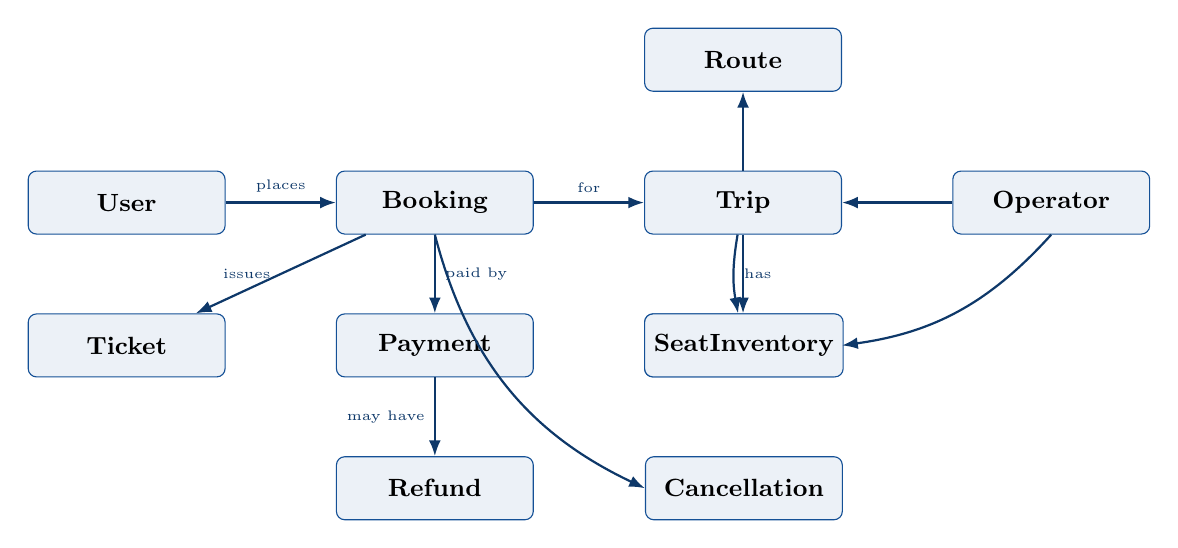
\begin{tikzpicture}[
   entity/.style={draw=busgoblue, fill=busgoblue!8, rounded corners=3pt,
                  minimum width=2.5cm, minimum height=0.8cm, font=\small\bfseries, align=center},
   rel/.style={-{Latex[length=2mm]}, busgoblue!70!black, thick},
   node distance=1.0cm and 1.4cm]

 \node[entity] (user) {User};
 \node[entity, right=of user] (booking) {Booking};
 \node[entity, right=of booking] (trip) {Trip};
 \node[entity, above=of trip] (route) {Route};
 \node[entity, below=of trip] (bus) {Bus};
 \node[entity, right=of trip] (operator) {Operator};

 \node[entity, below=of booking] (payment) {Payment};
 \node[entity, below=of user] (ticket) {Ticket};
 \node[entity, below=of payment] (refund) {Refund};
 \node[entity, right=of payment] (seat) {SeatInventory};
 \node[entity, below=of seat] (cancel) {Cancellation};

 \draw[rel] (user) -- node[above,font=\tiny]{places} (booking);
 \draw[rel] (booking) -- node[above,font=\tiny]{for} (trip);
 \draw[rel] (trip) -- (route);
 \draw[rel] (trip) -- (bus);
 \draw[rel] (operator) -- (trip);
 \draw[rel] (operator.south) to[bend left=20] (bus.east);
 \draw[rel] (booking) -- node[right,font=\tiny]{paid by} (payment);
 \draw[rel] (booking) -- node[left,font=\tiny]{issues} (ticket);
 \draw[rel] (payment) -- node[left,font=\tiny]{may have} (refund);
 \draw[rel] (trip) to[bend right=10] node[right,font=\tiny]{has} (seat);
 \draw[rel] (booking.south) to[bend right=25] (cancel.west);
\end{tikzpicture}
\end{center}

\textbf{Major relationships}
\begin{itemize}[leftmargin=1.4em]
  \item A \textbf{User} places many \textbf{Bookings}; each Booking references one \textbf{Trip}.
  \item A \textbf{Trip} belongs to one \textbf{Operator}, runs on one \textbf{Bus} along one \textbf{Route},
        and owns many \textbf{SeatInventory} rows.
  \item A \textbf{Booking} has one \textbf{Payment} and (on confirmation) one \textbf{Ticket}.
  \item A \textbf{Payment} may have one \textbf{Refund}; a \textbf{Booking} may have one \textbf{CancellationRequest}.
\end{itemize}

% =====================================================================
%  8. UI AND UX REQUIREMENTS
% =====================================================================
\section{UI and UX Requirements}

\subsection{Wireframes}
The following low-fidelity wireframes cover the primary passenger flow plus the operator portal.

% ---- Wireframe 1: Home / Search ----
\begin{center}
\textbf{Wireframe 1 — Home / Trip Search}\\[2pt]
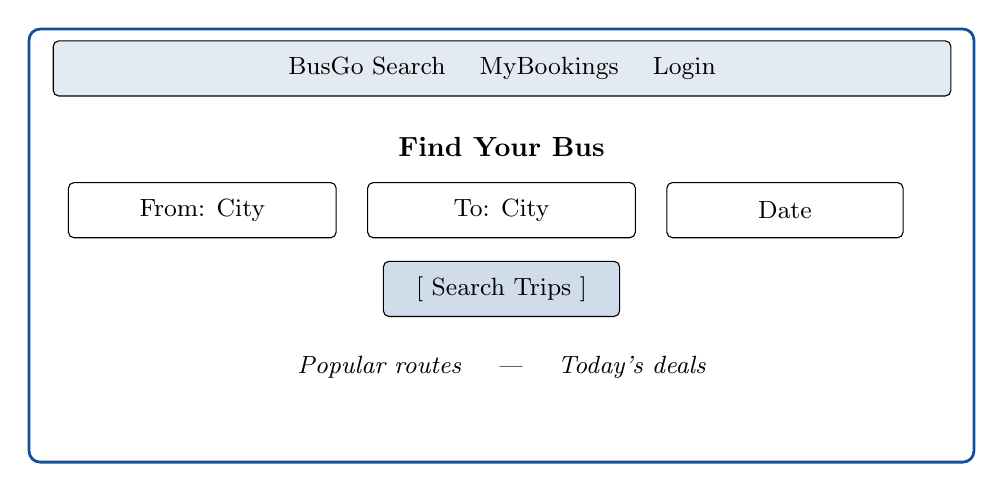
\begin{tikzpicture}[box/.style={draw, rounded corners=2pt, minimum height=0.7cm, font=\small}]
 \draw[draw=busgoblue, line width=1pt, rounded corners=4pt] (0,0) rectangle (12,5.5);
 \node[box, fill=busgoblue!12, minimum width=11.4cm, anchor=west] at (0.3,5){BusGo \hfill Search \quad MyBookings \quad Login};
 \node[font=\bfseries] at (6,4){Find Your Bus};
 \node[box, minimum width=3.4cm] at (2.2,3.2){From: City};
 \node[box, minimum width=3.4cm] at (6,3.2){To: City};
 \node[box, minimum width=3cm] at (9.6,3.2){Date};
 \node[box, fill=busgoblue!20, minimum width=3cm] at (6,2.2){[ Search Trips ]};
 \node[font=\small\itshape] at (6,1.2){Popular routes \quad | \quad Today's deals};
\end{tikzpicture}
\end{center}

% ---- Wireframe 2: Search results ----
\begin{center}
\textbf{Wireframe 2 — Search Results}\\[2pt]
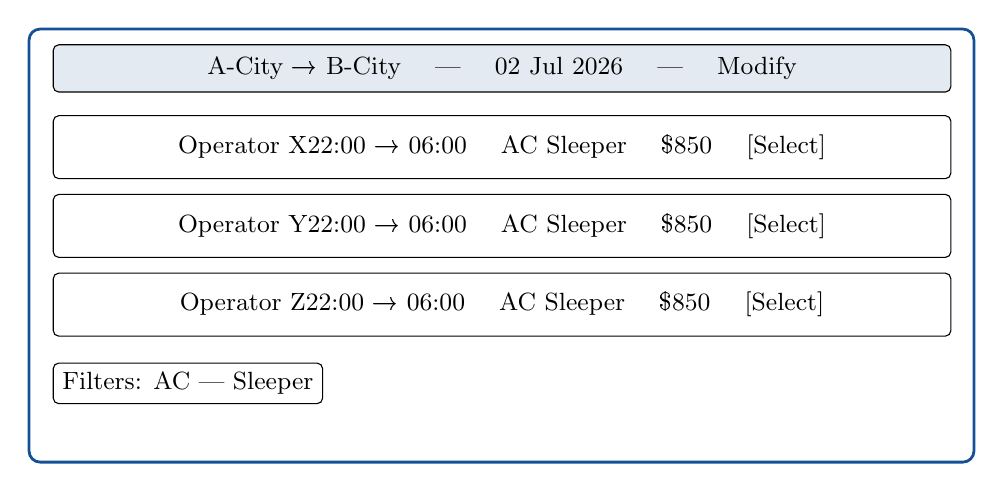
\begin{tikzpicture}[box/.style={draw, rounded corners=2pt, font=\small}]
 \draw[draw=busgoblue, line width=1pt, rounded corners=4pt] (0,0) rectangle (12,5.5);
 \node[box, fill=busgoblue!12, minimum width=11.4cm, minimum height=0.6cm, anchor=west] at (0.3,5){A-City \textrightarrow{} B-City \quad | \quad 02 Jul 2026 \quad | \quad Modify};
 \foreach \y/\op in {4/Operator X, 3/Operator Y, 2/Operator Z}{
   \node[box, minimum width=11.4cm, minimum height=0.8cm, anchor=west] at (0.3,\y){\op \hfill 22:00 \textrightarrow{} 06:00 \quad AC Sleeper \quad \$850 \quad [Select]};
 }
 \node[box, minimum width=3cm, anchor=west] at (0.3,1){Filters: AC | Sleeper};
\end{tikzpicture}
\end{center}

% ---- Wireframe 3: Seat selection ----
\begin{center}
\textbf{Wireframe 3 — Seat Selection}\\[2pt]
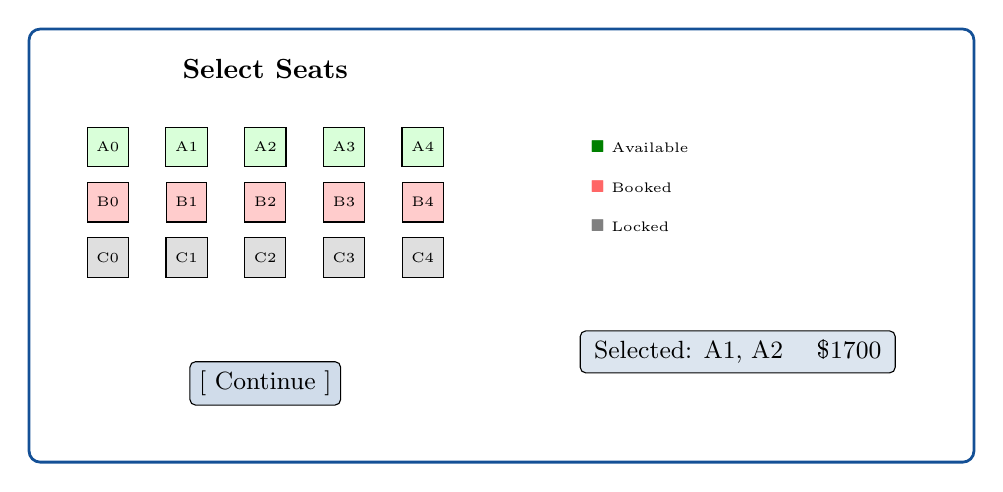
\begin{tikzpicture}[seat/.style={draw, minimum size=0.5cm, font=\tiny}]
 \draw[draw=busgoblue, line width=1pt, rounded corners=4pt] (0,0) rectangle (12,5.5);
 \node[font=\bfseries] at (3,5){Select Seats};
 \foreach \x in {0,1,2,3,4}{
   \node[seat, fill=green!15] at (1+\x,4){A\x};
   \node[seat, fill=red!20] at (1+\x,3.3){B\x};
   \node[seat, fill=gray!25] at (1+\x,2.6){C\x};
 }
 \node[font=\tiny, anchor=west] at (7,4){\textcolor{green!50!black}{$\blacksquare$} Available};
 \node[font=\tiny, anchor=west] at (7,3.5){\textcolor{red!60}{$\blacksquare$} Booked};
 \node[font=\tiny, anchor=west] at (7,3){\textcolor{gray}{$\blacksquare$} Locked};
 \node[draw, fill=busgoblue!15, rounded corners=2pt, minimum width=4cm, font=\small] at (9,1.4){Selected: A1, A2 \quad \$1700};
 \node[draw, fill=busgoblue!20, rounded corners=2pt, font=\small] at (3,1){[ Continue ]};
\end{tikzpicture}
\end{center}

% ---- Wireframe 4: Payment ----
\begin{center}
\textbf{Wireframe 4 — Passenger Details \& Payment}\\[2pt]
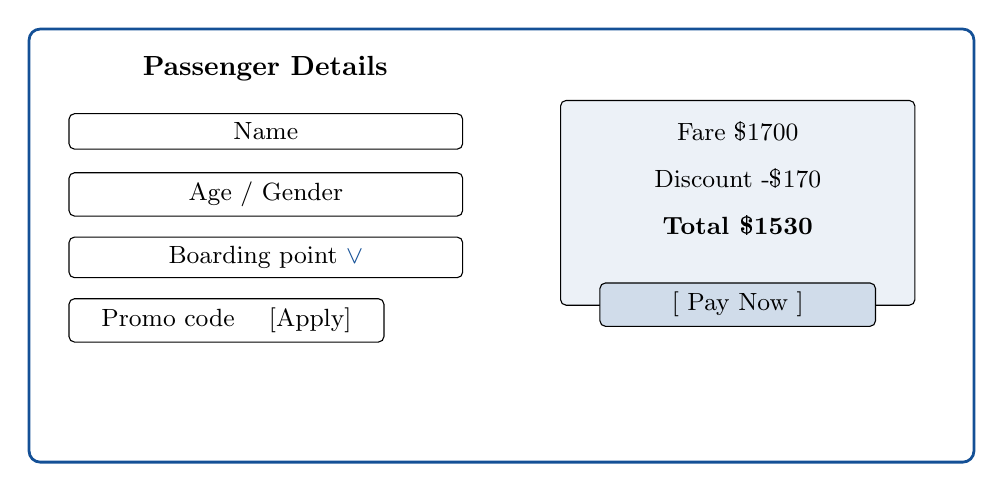
\begin{tikzpicture}[box/.style={draw, rounded corners=2pt, font=\small}]
 \draw[draw=busgoblue, line width=1pt, rounded corners=4pt] (0,0) rectangle (12,5.5);
 \node[font=\bfseries] at (3,5){Passenger Details};
 \node[box, minimum width=5cm, anchor=west] at (0.5,4.2){Name};
 \node[box, minimum width=5cm, anchor=west] at (0.5,3.4){Age / Gender};
 \node[box, minimum width=5cm, anchor=west] at (0.5,2.6){Boarding point \textcolor{busgoblue}{$\vee$}};
 \node[box, minimum width=4cm, anchor=west] at (0.5,1.8){Promo code \quad [Apply]};
 \node[draw, fill=busgoblue!8, rounded corners=2pt, minimum width=4.5cm, minimum height=2.6cm, anchor=north] at (9,4.6){};
 \node[font=\small] at (9,4.2){Fare \$1700};
 \node[font=\small] at (9,3.6){Discount -\$170};
 \node[font=\small\bfseries] at (9,3){Total \$1530};
 \node[box, fill=busgoblue!20, minimum width=3.5cm] at (9,2){[ Pay Now ]};
\end{tikzpicture}
\end{center}

% ---- Wireframe 5: Confirmation / Ticket ----
\begin{center}
\textbf{Wireframe 5 — Booking Confirmation \& E-Ticket}\\[2pt]
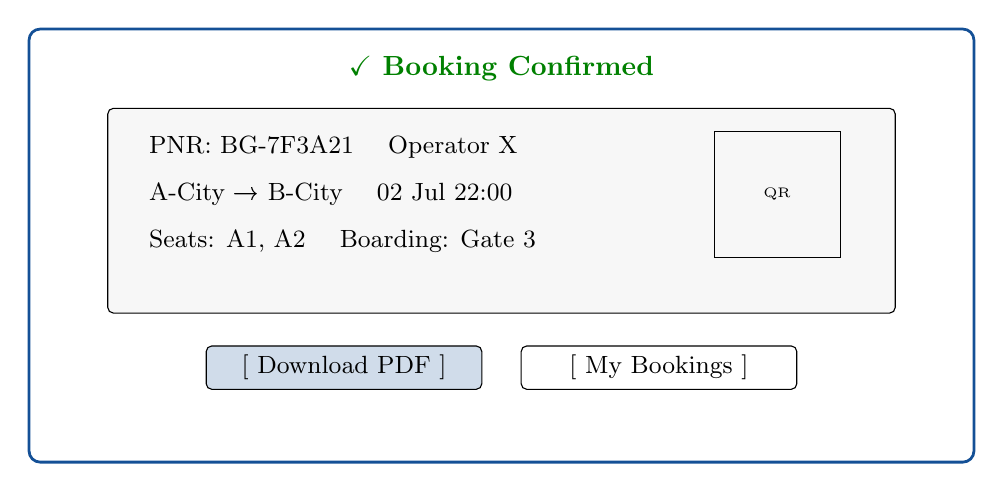
\begin{tikzpicture}[box/.style={draw, rounded corners=2pt, font=\small}]
 \draw[draw=busgoblue, line width=1pt, rounded corners=4pt] (0,0) rectangle (12,5.5);
 \node[font=\bfseries\color{green!50!black}] at (6,5){\checkmark{} Booking Confirmed};
 \node[draw, fill=black!3, rounded corners=2pt, minimum width=10cm, minimum height=2.6cm, anchor=north] at (6,4.5){};
 \node[font=\small, anchor=west] at (1.4,4){PNR: BG-7F3A21 \quad Operator X};
 \node[font=\small, anchor=west] at (1.4,3.4){A-City \textrightarrow{} B-City \quad 02 Jul 22:00};
 \node[font=\small, anchor=west] at (1.4,2.8){Seats: A1, A2 \quad Boarding: Gate 3};
 \node[draw, minimum size=1.6cm, font=\tiny] at (9.5,3.4){QR};
 \node[box, fill=busgoblue!20, minimum width=3.5cm] at (4,1.2){[ Download PDF ]};
 \node[box, minimum width=3.5cm] at (8,1.2){[ My Bookings ]};
\end{tikzpicture}
\end{center}

% ---- Wireframe 6: Operator portal ----
\begin{center}
\textbf{Wireframe 6 — Operator Portal (Manage Trips)}\\[2pt]
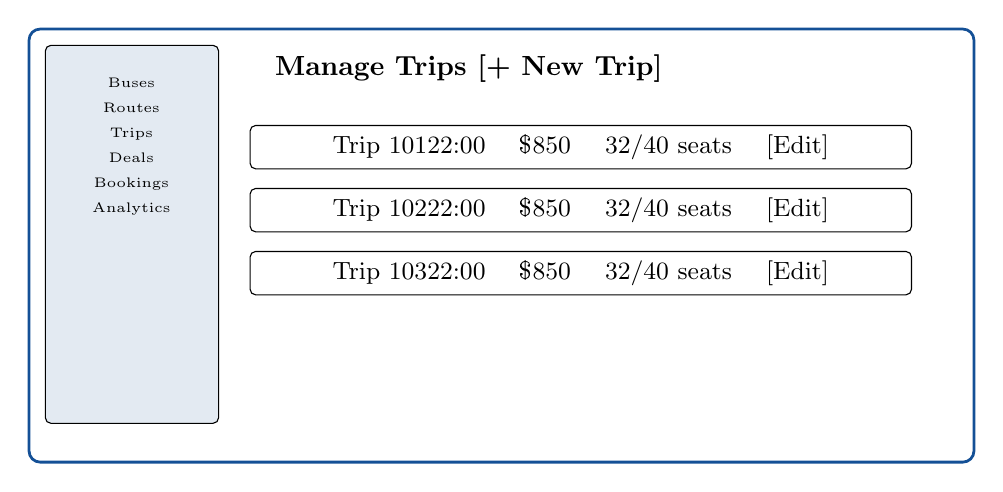
\begin{tikzpicture}[box/.style={draw, rounded corners=2pt, font=\small}]
 \draw[draw=busgoblue, line width=1pt, rounded corners=4pt] (0,0) rectangle (12,5.5);
 \node[box, fill=busgoblue!12, minimum width=2.2cm, minimum height=4.8cm, anchor=north west] at (0.2,5.3){};
 \node[font=\tiny, anchor=north, align=center] at (1.3,5){Buses\\[3pt]Routes\\[3pt]Trips\\[3pt]Deals\\[3pt]Bookings\\[3pt]Analytics};
 \node[font=\bfseries, anchor=west] at (3,5){Manage Trips \hfill [+ New Trip]};
 \foreach \y/\r in {4/Trip 101, 3.2/Trip 102, 2.4/Trip 103}{
   \node[box, minimum width=8.4cm, anchor=west] at (2.8,\y){\r \hfill 22:00 \quad \$850 \quad 32/40 seats \quad [Edit]};
 }
\end{tikzpicture}
\end{center}

\subsection{UX and Accessibility Baseline}
\begin{itemize}[leftmargin=1.4em]
  \item \textbf{Clear navigation and labels:} persistent top navigation; descriptive button labels
        (e.g., ``Search Trips'', ``Pay Now''); breadcrumb of the booking steps.
  \item \textbf{Keyboard accessibility:} all core flows (search, seat select, pay) operable via
        keyboard; visible focus states; logical tab order.
  \item \textbf{Readable contrast and typography:} WCAG AA contrast ($\geq 4.5{:}1$) for text;
        minimum 16px body text; colour is never the sole status indicator (seat states also
        labelled).
  \item \textbf{Responsive behavior:} layouts adapt from desktop to mobile widths; seat map and
        booking summary reflow on small screens.
  \item \textbf{Feedback:} loading states, inline validation messages, and toast notifications for
        success/error.
\end{itemize}

% =====================================================================
%  9. NON-FUNCTIONAL REQUIREMENTS
% =====================================================================
\section{Non-Functional Requirements}

NFR ID format: \texttt{NFR-T07-\#\#\#}.

\begin{longtable}{p{2.1cm} p{2.4cm} Y Y}
\toprule
\rowstyle \textbf{NFR ID} & \textbf{Category} & \textbf{Requirement} & \textbf{Target / Metric} \\
\midrule
\endhead
NFR-T07-001 & Performance & Trip search results shall return quickly under normal load. & p95 latency $\leq 800$\,ms for search at 50 concurrent users. \\
NFR-T07-002 & Performance & Seat map shall load promptly after trip selection. & p95 $\leq 1$\,s. \\
NFR-T07-003 & Scalability & Services shall scale horizontally behind the Kong gateway. & Each service runs $\geq 2$ replicas with load balancing. \\
NFR-T07-004 & Availability & Core booking path shall remain available during single-service restarts. & $\geq 99\%$ monthly availability in dev environment. \\
NFR-T07-005 & Reliability & Seat locks shall auto-expire to prevent permanent blocking. & 100\% of expired locks released within the lock window + 60\,s. \\
NFR-T07-006 & Consistency & Booking creation shall be idempotent. & Duplicate idempotency key never creates a second booking. \\
NFR-T07-007 & Security & Passwords shall be stored only as salted hashes. & 0 plaintext passwords; bcrypt with cost $\geq 12$. \\
NFR-T07-008 & Security & APIs shall require JWT auth for protected routes. & 401 returned for missing/invalid tokens. \\
NFR-T07-009 & Security & All client traffic shall pass through the API gateway. & No service is directly reachable by clients in deployment. \\
NFR-T07-010 & Usability & Core booking flow shall be completable in few steps. & $\leq 5$ screens from search to confirmation. \\
NFR-T07-011 & Accessibility & UI shall meet WCAG 2.1 AA basics. & Contrast $\geq 4.5{:}1$; keyboard operable core flows. \\
NFR-T07-012 & Maintainability & Each service shall be independently deployable. & Service can be rebuilt/restarted without redeploying others. \\
NFR-T07-013 & Observability & System shall expose metrics, logs, and health. & Prometheus metrics, Loki logs, \texttt{/health} per service. \\
NFR-T07-014 & Portability & Stack shall run via Docker Compose on a dev machine. & \texttt{make up} brings up all services. \\
NFR-T07-015 & Data Integrity & Audit log shall be append-only. & No update/delete on audit entries. \\
NFR-T07-016 & Recoverability & Services shall recover from transient Kafka/Redis outages. & Service restarts and reconnects without manual data fixes. \\
\bottomrule
\end{longtable}

% =====================================================================
%  10. RISKS AND OPEN QUESTIONS
% =====================================================================
\section{Risks and Open Questions}

\subsection{Risk Register}
\begin{longtable}{p{2.1cm} Y p{1.9cm} p{1.6cm} Y}
\toprule
\rowstyle \textbf{Risk ID} & \textbf{Description} & \textbf{Probability} & \textbf{Impact} & \textbf{Mitigation} \\
\midrule
\endhead
RISK-T07-001 & Distributed consistency: seat lock and booking span two services and may diverge. & Medium & High & Time-bound locks + idempotency keys + reconciliation job. \\
RISK-T07-002 & Kafka unavailability causes services to crash-loop on startup. & Medium & High & Retry/backoff on connect; health gating; documented recovery steps. \\
RISK-T07-003 & Schema changes require volume wipe (\texttt{create\_all}, no migrations). & High & Medium & Introduce Alembic migrations before production; seed scripts for reload. \\
RISK-T07-004 & Mock payment behaviour diverges from a real PSP. & High & Medium & Encapsulate gateway behind an interface for later swap. \\
RISK-T07-005 & Gateway misrouting (singular vs plural paths) breaks endpoints. & Medium & Medium & Kong config supports both forms; route tests in CI. \\
RISK-T07-006 & Port conflicts / Windows excluded-port bind failures in dev. & Medium & Low & Documented 850x port convention; configurable host ports. \\
RISK-T07-007 & Team capacity: four-member student team across timed labs. & Medium & Medium & Prioritise Must requirements; defer Could/Won't items. \\
RISK-T07-008 & Security: JWT/secret handling in dev may leak. & Low & High & Environment-based secrets; rotate keys; no secrets in repo. \\
\bottomrule
\end{longtable}

\subsection{Open Questions}
\begin{itemize}[leftmargin=1.4em]
  \item What exact refund policy tiers apply (time-before-departure brackets and percentages)?
  \item What is the precise seat-lock duration, and should it differ by trip popularity?
  \item Which mock payment methods must be supported in v1 (card, wallet, netbanking)?
  \item Should OAuth login be in v1 scope or deferred to a later release?
  \item What user segmentation is required for admin broadcast notifications?
  \item Is multi-seat-per-booking limited (e.g., max seats per transaction)?
\end{itemize}

% =====================================================================
%  11. TESTABILITY AND TRACEABILITY
% =====================================================================
\section{Testability and Traceability}

\subsection{Requirement Traceability}
\begin{longtable}{p{2.6cm} p{3.0cm} p{3.0cm}}
\toprule
\rowstyle \textbf{Requirement ID} & \textbf{Story / Use Case} & \textbf{Planned Test ID} \\
\midrule
\endhead
FR-T07-001 & US-T07-001 & TC-T07-001 \\
FR-T07-002 & US-T07-002 & TC-T07-002 \\
FR-T07-003 & US-T07-003 & TC-T07-003 \\
FR-T07-005 & US-T07-004 / UC-1 & TC-T07-004 \\
FR-T07-006 & US-T07-005 / UC-1 & TC-T07-005 \\
FR-T07-007 & US-T07-006 / UC-1 & TC-T07-006 \\
FR-T07-009 & US-T07-007 / UC-1 & TC-T07-007 \\
FR-T07-010 & US-T07-008 & TC-T07-008 \\
FR-T07-011 & US-T07-009 / UC-1 & TC-T07-009 \\
FR-T07-012 & US-T07-010 / UC-1 & TC-T07-010 \\
FR-T07-013 & US-T07-011 & TC-T07-011 \\
FR-T07-014 & US-T07-012 / UC-2 & TC-T07-012 \\
FR-T07-015 & US-T07-013 / UC-2 & TC-T07-013 \\
FR-T07-016 & US-T07-015 & TC-T07-014 \\
FR-T07-018 & US-T07-017 / UC-3 & TC-T07-015 \\
FR-T07-019 & US-T07-018 & TC-T07-008 \\
FR-T07-022 & US-T07-021 & TC-T07-014 \\
FR-T07-024 & US-T07-023 & TC-T07-013 \\
FR-T07-026 & UC-1 & TC-T07-009 \\
\bottomrule
\end{longtable}

\subsection{Initial Manual Test Plan}
\begin{longtable}{p{1.9cm} p{2.4cm} p{2.4cm} Y Y}
\toprule
\rowstyle \textbf{Test ID} & \textbf{Scenario} & \textbf{Preconditions} & \textbf{Steps} & \textbf{Expected Result} \\
\midrule
\endhead
TC-T07-001 & Register new user & Phone not registered & Submit registration form with valid data & Account created; OTP sent; 201 response. \\
TC-T07-002 & OTP verification & User registered, OTP issued & Enter valid OTP before expiry & Account marked verified. \\
TC-T07-003 & Login success & Verified user exists & Submit correct phone + password & JWT access \& refresh tokens returned. \\
TC-T07-004 & Trip search & Trips seeded for route/date & Search A-City \textrightarrow{} B-City for a future date & Matching trips with fares listed. \\
TC-T07-005 & Seat map load & A trip selected & Open seat map & Seats render with correct AVAILABLE/LOCKED/BOOKED states. \\
TC-T07-006 & Seat lock holds & Two sessions, same trip & Session A selects A1; Session B tries A1 & A1 unavailable to B until lock expiry. \\
TC-T07-007 & Create booking & Seats locked by user & Submit passenger details & Booking created in INITIATED with idempotency key. \\
TC-T07-008 & Apply valid promo & Active promo exists & Enter valid code at payment & Discount applied; total fare reduced. \\
TC-T07-009 & Successful payment & Booking INITIATED & Pay via mock gateway (success) & Booking CONFIRMED; payment SUCCESS. \\
TC-T07-010 & Ticket issued & Booking CONFIRMED & Open confirmation page & Unique QR ticket and PDF available. \\
TC-T07-011 & View my bookings & User has bookings & Open My Bookings & Bookings listed newest-first with status. \\
TC-T07-012 & Request cancellation & Confirmed booking exists & Submit cancellation with reason & PENDING request with computed refund amount. \\
TC-T07-013 & Approve refund & Pending cancellation exists & Support approves request & Refund record created; booking CANCELLED; seats released. \\
TC-T07-014 & Operator creates bus & Operator active & Add bus with unique registration & Bus saved; duplicate registration rejected. \\
TC-T07-015 & Operator schedules trip & Active bus \& route exist & Create trip with fare/capacity & Trip SCHEDULED; seat inventory generated. \\
TC-T07-016 & Duplicate registration & Phone already used & Register with same phone & 409 conflict; no duplicate account. \\
TC-T07-017 & Invalid login & Verified user exists & Submit wrong password & 401; no token issued. \\
TC-T07-018 & Expired promo rejected & Expired promo exists & Enter expired code & Code rejected with reason; no discount. \\
TC-T07-019 & Payment failure path & Booking INITIATED & Pay via mock gateway (failure) & Booking not confirmed; seats releasable. \\
TC-T07-020 & Gateway routing & Services up via Kong & Call \texttt{/api/search/...} & Request routed to Search service (200). \\
\bottomrule
\end{longtable}

% =====================================================================
%  12. SUBMISSION CHECKLIST
% =====================================================================
\section{Lab 2 Submission Checklist}
\begin{itemize}[leftmargin=2em, label=$\boxtimes$]
  \item Problem statement and scope are clear.
  \item Minimum 12 user stories with acceptance criteria (24 provided).
  \item Functional requirements table is complete (27 requirements).
  \item Data model and data dictionary are attached.
  \item Minimum 5 wireframes or flow screens included (6 provided).
  \item NFR section is completed (16 NFRs).
  \item Risks and open questions are documented.
  \item Initial manual test plan (15 cases) is included (20 provided).
\end{itemize}

\vfill
\begin{center}
\rule{0.5\textwidth}{0.4pt}\\[4pt]
{\small \textit{End of Document — BusGo SRS v1.0 — Team T07}}
\end{center}

\end{document}
